% THIS IS SIGPROC-SP.TEX - VERSION 3.1
% WORKS WITH V3.2SP OF ACM_PROC_ARTICLE-SP.CLS
% APRIL 2009
%
% It is an example file showing how to use the 'acm_proc_article-sp.cls' V3.2SP
% LaTeX2e document class file for Conference Proceedings submissions.
% ----------------------------------------------------------------------------------------------------------------
% This .tex file (and associated .cls V3.2SP) *DOES NOT* produce:
%       1) The Permission Statement
%       2) The Conference (location) Info information
%       3) The Copyright Line with ACM data
%       4) Page numbering
% ---------------------------------------------------------------------------------------------------------------
% It is an example which *does* use the .bib file (from which the .bbl file
% is produced).
% REMEMBER HOWEVER: After having produced the .bbl file,
% and prior to final submission,
% you need to 'insert'  your .bbl file into your source .tex file so as to provide
% ONE 'self-contained' source file.
%
% Questions regarding SIGS should be sent to
% Adrienne Griscti ---> griscti@acm.org
%
% Questions/suggestions regarding the guidelines, .tex and .cls files, etc. to
% Gerald Murray ---> murray@hq.acm.org
%
% For tracking purposes - this is V3.1SP - APRIL 2009

\documentclass{acm_proc_article-sp}
\usepackage{epstopdf}
\usepackage{amsmath}
\usepackage{bm}
\usepackage{enumitem}
\usepackage{commath}
\usepackage{xcolor}
\usepackage{graphicx}
\usepackage{natbib}
\usepackage{url}

\begin{document}

\title{A Survey of Recommendation Systems}
\numberofauthors{3} 
\author{
% 1st. author
\alignauthor
Shobhit Chaurasia\\
       \affaddr{11010179}\\
       \affaddr{Indian Institute of Technology Guwahati}\\
       \email{c.shobhit@iitg.ernet.in}
% 2nd. author
\alignauthor
Harshil Lodhi\\
       \affaddr{11010121}\\
       \affaddr{Indian Institute of Technology Guwahati}\\
       \email{harshil@iitg.ernet.in}
}

\maketitle
\begin{abstract}
A recommendation system tracks previous activities of a set of users, and analyses their purchasing, browsing or rating patterns to predict and recommend a set of items to each user which are potentially of interest to him. This paper provides an overview of the rapidly emerging field of recommender systems. We discuss the 3 main categories of recommendation systems: collaborative, content-based and hybrid systems. The paper also analyses standard algorithms for item-based recommendations, wherein recommendations are provided based on past activities of the user himself, and user-based recommendations, which computes similarities and relationships between different users and exploits these relationships to come up with recommendations. Further, we explore the state-of-the-art and variations to standard techniques employed in the current generation of recommender systems. Finally, we analyse their limitations and provide directions for future work.
\end{abstract}

\keywords{Recommendation Systems, Collaborative Filtering, Content-based Recommendations, User Based, Item Based} 
\section{Introduction}
Recommender systems has been a hot research topic since 1990s [c]. A lot of research has been done over the past two decades both in industry and in academia. With data growing at an enormous rate [c] (thanks to WWW), researchers are now trying to find out new ways to utilize the available data to extract out meaningful information.  Recommender systems has been an area of high interest because of high application in e-commerce and advertisement industry products. Today almost all the big websites depend on recommender systems for suggesting ads, products, articles, movies, videos etc. to their users. Examples include book suggestions on Amazon, movie recommendation on Netflix, Video recommendations on YouTube etc, product recommendation of Flipkart, question/answer recommendations on Quora. 

Over the past two decades, a lot of different approaches have been used. Collaborative filtering is one of the most widely used approach in the making of a recommender system. It works by finding similar users and then recommending items that are liked by similar users. This approach is called \textit{user-based approach}. Another common approach in building of recommender systems is to employ filtering based on content. In content based filtering, a description of products is constructed (in the form of item matrix) based on keywords and tags. Similarly a user profile is created to indicate what a particular user likes. Then the system tries to find items similar to those that user has liked/purchased in the past. This approach is called \textit{item-based approach}. In the recent years, researchers have tried to come up with a \textit{Hybrid approach} which tries to combine collaborative filtering and content based filtering. 

However, even after a couple of decades of work in the area of recommendations, the present generation of recommendation systems require deeper investigation and research so as to make them more accurate and effective. The shortcomings of today's recommendation systems can be attributed to the enormous amount of information pervading the Internet, not only in terms of size of content, but also its variety, spectrum and diversity. Potential improvements to current methods include broadening the domain for generating user profile by analysing his activities on different social platforms, improving item-profile modelling by incorporating user feedback and contextual information (such as higher weightage to FIFA franchise items during FIFA World Cup), and building more reliable evaluation metrics. 

In this paper, we present a survey of overview and background of recommendation systems in Section- 2, followed by a discussion of standard techniques used in recommendation systems in Section - . In Section - , we explore the state-of-the-art. Finally, we conclude by proposing directions for future work. 
\section{Overview of Recommender Systems}
Origin of recommendation systems can be traced back to work in cognitive science [1:87], principles of forecasting [1:6] and study of marketing models [1:60]. The formal research in recommendation systems kicked off in 1990s where the backbone of recommendations was the rating framework. The problem was perceived as the problem of rating estimation for undiscovered items for a user, based on his interests, past-purchases/activities; later [38] proposed the inclusion of activities of other users with similar interests as a parameter.

[1:45], [2:86], [3:97] provided mathematical formulation for the recommendation problem. Mathematically, the recommendation system can be formalized as follows: let $\textbf{U}$ denote the user space comprising of millions of users and $\textbf{I}$ denote the item-space encompassing millions of items to be recommended. Let $r:U\times I\rightarrow R$ denote the relevance function that captures the potential relevance of an item $i\in \textbf{I}$ to a user $u\in \textbf{U}$, where $R$ represents the set of real numbers, quantifying the relevance quotient. For each user $u\in \textbf{U}$, the problem of recommendation boils down to returning a set of top-$n$ items $i'\in \textbf{I}$ that maximizes the relevance function, i.e.
\begin{equation}
~i'\in\max_{\forall i\in I}r(u,i)
\end{equation}
The most commonly used relevance function $r$ is the ratings provided by the user on a predetermined scale. The core problem in recommendation systems is to \textit{learn} the relevance measure for item $i$ which is either undiscovered or unrated by user $u$. Recommendation techniques can be classified into 3 main categories as follows, based on the underlying principle used to estimate the ratings:
\begin{itemize}
\item \textit{Collaborative filtering techniques} leverage the ratings of items by a set of users having similar tastes and interests as the given user $u$, and recommend items to $u$ based on these analysis. This techniques requires generation of user profiles and item profiles, and employs different similarity metrics to gauge the similarity of two users. 
\item \textit{Content-based recommendations} employ measures which are local to a user $u$. It recommends items to the user based on his own browsing/rating/purchasing patterns in the past. It envisages the recommendation problem as a search for related items [cite 6th paper], learning the user's tastes by analysing past activities and recommending items related to his past purchases. Here also, similarity measures are applied on item profiles to quantify similarity of two items.
\item \textit{Hybrid techniques} combines the collaborative and content-based methods to build more robust and accurate recommendation systems.
\end{itemize}
Before diving into the technicalities of the above methods, we will explore few similarity measures commonly used to quantify the \textit{closeness} of two item-item/user-user/item-user profiles.
\section{Similarity}
Similarity of two items is defined as their \textit{closeness}. In Euclidean geometry, similarity of 2 points (vectors) $p_1=(\alpha_{11}, \alpha_{12},\dots,\alpha_{1n})$ and $p_2=(\alpha_{21}, \alpha_{22},\dots,\alpha_{2n})$ can be measured by calculating the Euclidean distance $d_E(p_1,p_2)$ as:
\begin{equation}
d_E(p_1,p_2) = \sqrt{(\alpha_{11}-\alpha_{21})^2+\dots +(\alpha_{1n}-\alpha_{2n})^2} \nonumber
\end{equation}
Another measure in Euclidean space is the \textit{$L_r$-norm} given by:
\begin{equation}
L_r(p_1,p_2) = (\displaystyle\sum_{i=1}^n \abs{\alpha_{1i}-\alpha_{2i}}^r)^{1/r}
\end{equation}
The \textit{$L_2$-norm} is same as the Euclidean Distance. A common measure in Euclidean space is the Manhattan Distance which is the \textit{$L_1$-norm}. These measures work well when the attributes of the two vectors have numerical values. However, in case of nominal attributes, such as gender (male, female), hair colour (black, brown, red, etc.) or ordinal attributes such as shirt size (small, medium, large, etc.), these trivial measures for computing similarity fail. To this end, measures such as Cosine Similarity and Pearson Correlation Similarity have been used \cite{almazro:survey}.

\begin{figure}[ht]
\centering
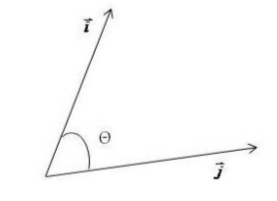
\includegraphics[height=0.35\columnwidth]{cosine}
\caption{The more the angle between the feature vectors, the lesser their similarity.}
\label{fig:cosine}
\end{figure}
\subsection{Cosine Similarity}
Items are represented as $m$ dimensional vectors (called feature vector), where each attribute represents a feature of the item. Items are characterized by the ordered set of values assigned to each feature. The similarity can then be viewed as the cosine of the angle between the two feature vectors as shown in Fig. \ref{fig:cosine}. Mathematically, it is defined as:
\begin{equation}
sim(\vec{a},\vec{b})=\cos\theta=\frac{\vec{a}\cdot\vec{b}}{\norm{\vec{a}}\cdot\norm{\vec{b}}}
\end{equation}

\subsection{Pearson Correlation Similarity}
Pearson Correlation Similarity measures correlation between two variables by computing the ratio of their co-variance and standard deviations. It is defined as:
\begin{equation}
p(x, y)=corr(x, y)=\frac{cov(x, y)}{\sigma_x\cdot\sigma_y} \nonumber
\end{equation}
In the domain of recommendation systems, it is used to find the correlation between items and users. Assume that both the items $a$ and $b$ have been rated by a set of users S. Let $R_{s,a}$ represent the rating given by user $s$ to item $a$. Further, let $\overline{R_a}$ denote the average rating for item $a$ over the complete user-space (who have rated $a$). The similarity measure is, then, defined as:
\begin{equation}
sim(a,b)=\frac{\sum_{s\in S} (R_{s,a}-\overline{R_a})(R_{s,b}-\overline{R_b})}{\sqrt{\sum_{s\in S} (R_{s,a}-\overline{R_a})^2}\sqrt{\sum_{s\in S} (R_{s,b}-\overline{R_b})^2}}
\end{equation}





\bibliographystyle{plainnat}
\bibliography{paper}
\end{document}
